\chapter{Introduction}
Particle accelerators occupy a key role both in fundamental research and in all the applications and industrial processes that uses technology and processes developed initially for the physical research. E.g. at the moment there is a huge demand of high brilliance light sources, that are fundamental to inquire all the phenomena which take place at the nanoscale. In this perspective keep developing the accelerators for the physical research is a fundamental requirement to assure that the cutting-edge technology of today turns into the labware of tomorrow for all the other sciences, in addition of the contribution that pursuing the fundamental research can give to our understanding of the microscopic world.

At the moment the most successful model to explain the behaviour of the elementary particles is the \textit{Standard Model}, but it's not conclusive and not able to answer to all the questions still open in particle physics. A milestone in favour of the Standard Model was the observation of the Higgs Boson in 2012, and was made possible by the construction of the \textit{Large Hadron Collider} at CERN\cite{CMS:higgs,ATLAS:higgs,LHC:design}. However the full understanding of the physics at the particle scale still needs to be achieved. Partially this will be realised with the increase of the collision energy of the LHC, but also the International Committee for Future Accelerators (ICFA) consider that the results of LHC needs to be complemented by the results of a lepton collider in the TeV-range\cite{ICFA:linStat}.

The reason of this decision is that according to the standard model the hadrons are particles composed by quarks, that are continously interacting exchanging gluons. This peculiarity cause the collision at high energy not to be between the hadrons themselves, but within the quarks that are composing them. In addition, there energy of the quarks are distributed statistically, so it's not possible to know in advance which will be the energy of the collision. On the other hand, the leptons are punctual particles, so the interaction is directly involving the two bullets themselves, and the number of possible processes that can take place is definitely smaller. 
This behaviour of particles of different kinds makes hadron colliders \textit{machines for discovery}, because involve all the possible processes that can take place, and the lepton machines \textit{machines for precision}, because the reduced number of possible processes guarantees the observation of the events of interest much easier.

In a collider the probability of observe a particular interaction process is given by
\[
P = \mathscr{L} \sigma
\]
where $\sigma$ is the process cross-section, which depends by the physics of the process itself, and $\mathscr{L}$ is the luminosity, which depends entirely by the machine.
Therefore the figure of merit when it comes to talk about accelerators is the luminosity, which is given by
\[
\mathscr{L} = H_d \frac{N^2}{\sigma_x \sigma_y} n_b f_r
\]
where $N$ is the number of particles per bunch, $\sigma_x$ and $\sigma_y$ are the beam dimensions in the horizontal and vertical plane, $n_b$ is the number of particle per bunch, $f_r$ is the collision frequency of the bunches and $H_d$ is a correction factor that takes in account the non ideality of the collision, such as crossing angle, collision offset, hour glass effect, non gaussian beam profile and so on.

Then becomes obvious try to reach the highest luminosity possible since the events that are going to be studied are rare. This is realised using two kinds of machines:
\begin{itemize}
\item linear accelerators (LINACs): present a low repetition frequency, typically lower than hundred of Hz and the beam is passing just once to be accelerated through the machine.
\item circular accelerators (typically synchrotrons): have a higher repetition frequency, up to tenth of KHz, and are keeping the particle beam in orbit for many turns, so can accelerate it over a long period of time
\end{itemize}
The key issue in the realisation of a lepton circular collider is the emission of synchrotron radiation, and is known that the power irradiated by a single particle in a circular machine scales according to the law
\[
P \propto \frac{1}{\rho^2} \frac{E^4}{m_0^4}
\]
where $\rho$ is the bending radius of the machine, $E$ is the particle energy and $m_0$ is its rest mass. As can be noted in the table 1.1, the energy loss per turn is a relevant fraction of the beam energy, e.g for the LEP machine over than 3 GeV were lost per turn, while the record energy per beam was 104.5 GeV. To raise the beam energy and combat the energy loss, the radius of circular machines escalates quickly. Simply scaling LEP, it is possible to show that in order to reach the centre-of-mass energy of 3 TeV, the circumference should be increased to thousands of kilometers \cite{nature:CLIC}.
To solve the issue the development of new lepton colliders is so focusing on two different solutions:
\begin{enumerate}
\item Use muons instead of electrons: this approach has to deal with the short life of muons, which is roughly $2 \, \mu s$ in the laboratory frame
\item Limit the losses caused by synchrotron radiation, or increasing the bending radius or abandon the circular topology for the linear one
\end{enumerate}
Also has to be noted that the former technology is rather new and needs to still be fully developed, while the latter profits of the progresses achieved in the last half century mainly in SLAC and KEK on the LINAC technology.

In this perspective a number of project are under study at the moment, of wich the most ambitious are FCC-ee,\textit{Future Circular Collider}, ILC, \textit{International Linear Collider}, and CLIC, \textit{Compact Linear Collider}. The first one consist in a circular collider which is supposed to be placed in a 80-100 km long tunnel before of the installation of the FCC-hh, the other are LINACs even if based on completely different technologies and solutions.  A comparison of the features of these projects in the final stage is presented in the table \ref{table_CLIC_ILC_FCC}, and also LEP is presented as example of circular lepton machine.

\begin{table}
  \centering
    \begin{tabular}{ l c c | c c c }
    \hline
    \hline
    Parameter								& LEP2	&	FCC-ee	&  \multicolumn{2}{c}{CLIC}	&	ILC	\\
    \hline
    $\sqrt{s} \, [GeV]$				& 209	& 350  		&  	500	&  3000	& 500	\\
    $\mathscr{L}_{peak}$  $[10^{34} \, cm^{-2} \, s^{-1}]$	&0.012	& 1.3			&  	2.3	& 	5.9	&1.8		\\
    Total lenght $[km]$						&26.7	& 100		& 13		&  48.4	& 31		\\
    Loaded acc. gradient $[MV/m]$				&		& 			& 80		& 100 	& 31.5	\\
    Bunch population $[10^9]$					& 105	& 170  		&  6.8	& 	3.72	& 500	\\
    Bunch spacing $[ns]$						& 		& 4000	  	&  	0.5	& 	0.5	& 554	\\
    Number of bunches						& 4		&  			&  		& 		& 1312	\\
    Collision rate $[Hz]$						&  		&  			&  	50	& 	50	& 5		\\
    $\epsilon^*_x \, / \, \epsilon^*_y \, [\mu m]/[nm]$	& 		&  		        &  2.4/25	& 0.66/20	& 10/35	\\  
    $\sigma^*_x\, / \, \sigma^*_y\, [nm]$			& 		&  	3600/70	&  202/2.3	& 40/1	&474/5.9	\\    
    Energy loss per turn $[GeV]$					&  3.34	& 	7.55		& - 		& -		& -		\\
    Power consumption $[MW]$					&  3.34	& 	7.55		& 		& 		& 163	\\
    \hline
    \hline
    %%%%%%%%%%%TABLE STILL TO FIX
    \end{tabular}
  \caption{Comparison of two circular machines, LEP\cite{FCC-ee:leptonCollParam} and FCC-ee\cite{FCC-ee:leptonCollParam,Zimmermann:2057706} and the two projects for linear machines, the fist and last stage of the CLIC implementation \cite{CLIC:cdr} and the final stage of ILC\cite{ILC:tdr} }
\label{table_CLIC_ILC_FCC}
\end{table}



Furthermore a recent interest arose on more compact technologies, e.g. plasma acceleration techniques, but the reliability of such designs still need to be proven in the perspective of creating a fully functional machine that goes beyond the demonstration of the working physical principle.







\newpage
\section{The CLIC poject and the CTF3 facility}

\begin{center}
\textit{still to do}
\end{center}
%goal 3 TeV, staging

%bunch structure (pag 2 of CDR update 2016 on staging),  and less than one interacting. So detector challenging

\subsection{Physics and staging}

The machine is designed to be built in 3 stages, with a final energy of 3 TeV. The energy of the stages have been chosen in order to offer a comprehensive physics programme, that is mainly focused on Higgs boson and top quark physics. This modular scheme should allow a physics programme that last for several decades.

Since the CDR\cite{CLIC:cdr} was released just before the discovery of the Higgs boson, the centre of mass energy stages have been reshaped in order to be able to access to interesting measurements on both Higgs and Top physics. Anyway for a given centre-of-mass energy, the energy can be modified by a third with limited loss of performance\cite{CLIC:cdrVol3}, allowing an eventual retuning of the energy of the stages following the results of the last LHC physics campaign.

The energy staging have been chosen as follows, further informations can be found in\cite{CLIC:staging2016,Bozovic-Jelisavcic:2160172}. As reference is useful to keep in mind the behaviour of the cross sections of the processes involving the Higgs boson, that are presented in figure \ref{higgs_cs} as function of the centre-of-mass energy.

The first stage is proposed to be 380 GeV, and it gives access to the Standard model Higgs physics and top-quark physics. The measurements on the former can be conducted through Higgsstrahlung and WW-fusion processes, thereby providing accurate model-indipendent measurements of Higgs couplings to bosons and fermions\cite{Roloff:2210491}; the latter measurements will be focused on the $t\bar{t}$ pair production threshold in the vicinity of $\sqrt{s} = $ 350 GeV.

The second stage is proposed at 1.5 TeV and allows to access new physics phenomena and additional properties of the Higgs boson and the top quark, such as Higgs self-coupling and rare Higgs branching ratios.

The third stage is proposed at 3 TeV and will give direct access to pair-produced particles with mass up to 1.5 TeV or single particles with mass up to 3 TeV. This stage is particularly interesting as test for the BSM theories, since such high energy in a lepton machine makes the observation of new particles much easier than in the LHC.

\begin{figure}
\centering

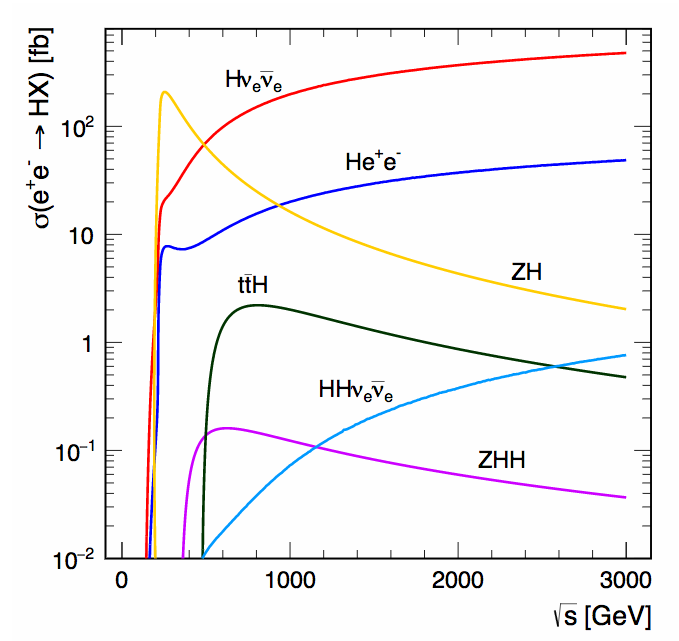
\includegraphics[scale=0.35]{pictures/higgs_cs}
\caption{Cross section dependence by the centre-of-mass energy of the most common processes involving the Higgs boson in a $e^+ e^-$ collider}
\label{higgs_cs}
\end{figure}

%% ADD HIGGS BOSON MOST COMMON PROCESSES 
% e+e- -> ZH
% e+e- -> Hvv
% e+e- -> He+e-
%%%%%%%%%% + TABLE OF CROSS SECTIONS AND FEYNMAN DIAGRAMS


%% BUT TOP PHYSICS ????



\subsection{The two beam acceleration concept}

In lobortis augue porta dui venenatis sollicitudin. In sagittis quis ipsum non dictum. Sed tempus, quam non vehicula dictum, mauris nisl posuere metus, eu lobortis odio risus at dui. Nullam non ante vulputate nulla ultrices euismod eu a diam. Cum sociis natoque penatibus et magnis dis parturient montes, nascetur ridiculus mus. Nulla nec augue a risus viverra mattis. Ut tincidunt egestas nulla at semper. Fusce pretium, leo quis consectetur viverra, arcu lectus ornare leo, quis commodo ex risus sit amet velit. Nullam finibus lorem in mi tincidunt, sed feugiat lectus tincidunt. In hac habitasse platea dictumst. Sed quis auctor odio, at sodales nunc. Donec vulputate massa sit amet dolor sollicitudin, vel pretium quam scelerisque. Nullam et massa eleifend, venenatis ante vitae, ornare libero. Suspendisse potenti. Nam ante lacus, porttitor vel turpis quis, pellentesque auctor velit.

In lobortis augue porta dui venenatis sollicitudin. In sagittis quis ipsum non dictum. Sed tempus, quam non vehicula dictum, mauris nisl posuere metus, eu lobortis odio risus at dui. Nullam non ante vulputate nulla ultrices euismod eu a diam. Cum sociis natoque penatibus et magnis dis parturient montes, nascetur ridiculus mus. Nulla nec augue a risus viverra mattis. Ut tincidunt egestas nulla at semper. Fusce pretium, leo quis consectetur viverra, arcu lectus ornare leo, quis commodo ex risus sit amet velit. Nullam finibus lorem in mi tincidunt, sed feugiat lectus tincidunt. In hac habitasse platea dictumst. Sed quis auctor odio, at sodales nunc. Donec vulputate massa sit amet dolor sollicitudin, vel pretium quam scelerisque. Nullam et massa eleifend, venenatis ante vitae, ornare libero. Suspendisse potenti. Nam ante lacus, porttitor vel turpis quis, pellentesque auctor velit.



